 \documentclass[a4paper,12pt]{report}

\usepackage{alltt, fancyvrb, url}
\usepackage{graphicx}
\usepackage[utf8]{inputenc}
\usepackage{float}
\usepackage{hyperref}

% Questo commentalo se vuoi scrivere in inglese.
\usepackage[italian]{babel}

\usepackage[italian]{cleveref}

\title{Relazione per\\``Programmazione ad Oggetti''\\Stubborn}

\author{Mario Ciccioni, Andrea Bianchi, Alessandro Cacciaguerra}
\date{\today}


\begin{document}

\maketitle

\tableofcontents

\chapter{Analisi}

Il software, un videogioco 2D bird-eye view survival, proporra' al videogiocatore un'esperienza di un classico videogame survival dove lo scopo e' quello di resistere il maggior tempo possibile cercando anche di accumulare punti durante la partita.
Il videogiocatore avra' la possibilita' di muoversi nel mondo di gioco con il suo personaggio, sopravvivere ai nemici che incontrera' nella mappa, raccogliere oggetti e recuperare vita.
Per bird-eye view si intende una visuale dall'alto del mondo di gioco.

\section{Requisiti}

\subsubsection{Requisiti funzionali}
\begin{itemize}
	\item Una volta avviato il software verra' presentato a schermo un menu' di gioco dove il videogiocatore potra' scegliere se iniziare una nuova partita, visualizzare la classifica dei punteggi o uscire dall'applicazione.
    \item La partita termina solo quando il personaggio perdera' tutte le vite a sua disposizione.
\end{itemize}

\subsubsection{Requisiti non funzionali}
\begin{itemize}
	\item Stubborn dovra' garantire una buona gestione delle risorse, non presentare lag pesanti in grado di rovinare l'esperienza di gioco e una grafica che permetta il chiaro riconoscimento di oggetti di gioco e nemici sparsi per la mappa.
    \item Tutte le informazioni relative alla partita in corso saranno mostrate a schermo in modo intuitivo, senza essere troppo invasive ma allo stesso tempo facimente controllabili anche durante la partita. 
\end{itemize}

\section{Analisi e modello del dominio}
Il videogioco denominato Stubborn proporra' al giocatore alcune semplici challenge, alcune di esse saranno implementate mentre altre lo sarano in futuro.
In particolare il giocatore avra/' la possibilita/' di raccogliere oggetti collezionabili che si trovano sulla mappa fin dall'inizio della partita ed al tempo stesso non deve prendere danno dai nemici.
Il player ha a disposizione 3 vite, se verra/' colpito da un nemico ne perdera/' una.
La fine del gioco avverra/' solo quando il player finira/' le vite a sua disposizione.
Riguardo ai nemici, essi verranno spawnati nella mappa di gioco con una logica random, a inizio partita, mentre per quanto riguarda la loro Ai puo' essere random oppure focalizzata sull'inseguimento del player.
Alcune funzionalita/' come diverse implementazioni di Ai nemici, attacco player > nemici, gameover ecc. verranno implementate in futuro e quindi il software sara' progettato in modo da apliare lo stesso in un futuro in modo semplice e veloce.
Di seguito viene mostrato lo schema UML dell'anali del problema contenenete le entita' principali che costutuiscono il problema \Cref{img:analysisUML}.

\begin{figure}[H]
\centering{}
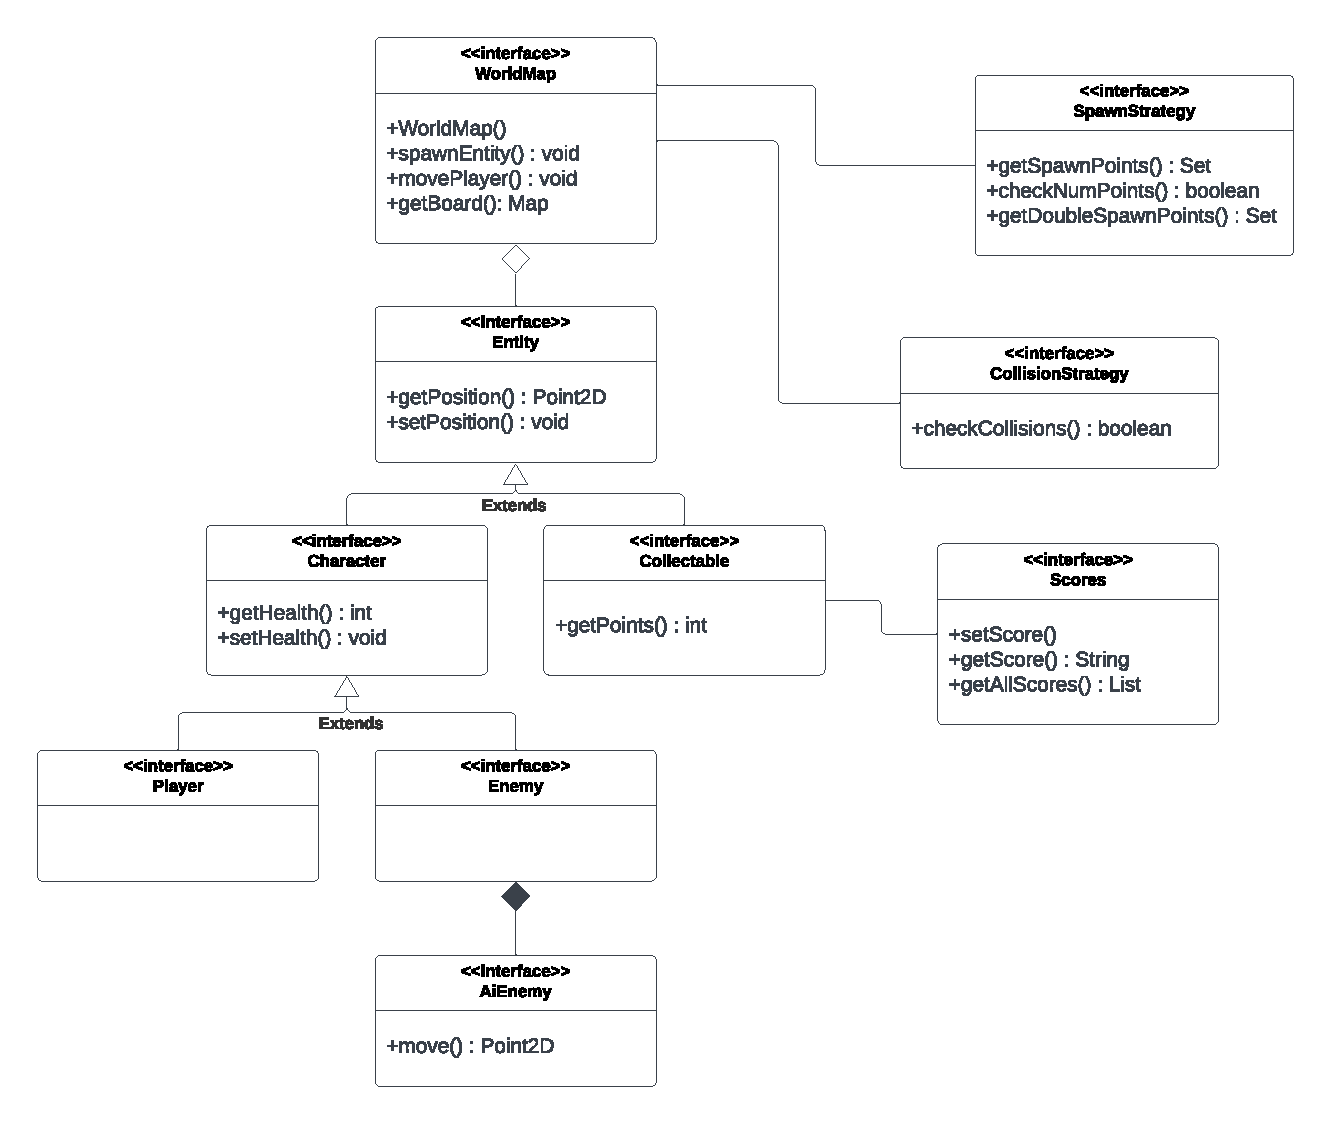
\includegraphics[width=\textwidth,height=\textheight,keepaspectratio]{img/analysisUML.pdf}
\caption{Schema UML dell'analisi del problema, con rappresentate le entità principali ed i rapporti fra loro **DA AGGIORNARE**}
\label{img:analysisUML}
\end{figure}

\chapter{Design}

\section{Architettura}
Il pattern architetturale scelto per la realizzazione del software e' MVP (Model View Presenter). In particolare abbiamo adottato la variante MVP Passive View, ossia la view e' un componente completamente passivo del sistema e non svolge nessuna operazione ma viene solo aggiornata dai Controller.
L'entry point del model e' WorldMap, essa e' la main class del software che contiene la logica generale del videogioco. Per quanto riguarda i Controller abbiamo deciso di adottare una logica di divisione dello stesso. Per ogni macro compito del software abbiamo implementato un suo specifico Controller in grado di comunicare con la view e se necessario comunicare con/modificare lo stato del model.
% Entry point della view ??? da aggiungere ???
I principali vantagggi dell'adottare questa architettura sono i seguenti:
\begin{itemize}
	\item Fornire al software una maggiore modularita', offrendo la possibilita' di cambiare parti di codice senza interferire con la logica del sistema. 
    \item E' possibile cambiare libreria grafica senza che essa impatti sul Controller, ne tantomeno sul Model ( la logica del sistema non risentira' in alcun modo di questi cambiamenti) 
\end{itemize}
% schema UML generale di interazione tra Controller e Model

\section{Design dettagliato}
\textbf{ANDREA BIANCHI}
\\ \\
\textit{Generazione/Posizionamento delle entità all’interno della mappa di gioco}
\begin{itemize}
    \item \textbf{Problema:} : La corretta generazione del posizionamento del protagonista, dei nemici e degli oggetti raccoglibili (entità), che saranno collocati all’interno della mappa di gioco.
    \item \textbf{Soluzione:} Il sistema utilizza Pattern Strategy, rappresentato dall’ interfaccia SpawnStrategy: questo approccio ci permette di disaccoppiare l’effettiva mappa di gioco dalle diverse  possibili implementazioni e variazioni su come verranno generati i punti dove saranno collocate le entità di gioco; si offre così una grande estendibilità utile ad ulteriori implementazioni e variazioni anche più complesse.
\end{itemize}

\textit{Interazioni tra le varie entità e con i confini della mappa di gioco.}
\begin{itemize}
    \item \textbf{Problema:} Entità in grado di muoversi all’interno della mappa, quali il giocatore e il nemico, rischiano di riuscire a superare i confini della mappa o di raggiungere entrambi una stessa posizione, questo rende necessario lo sviluppo di un sistema di collisioni.
    \item \textbf{Soluzione:} Il sistema si avvale nuovamente del Pattern Strategy, tramite l’interfaccia CollisionStrategy:  questo sistema offre una forma di riuso di codice per gestire eventi di collisione comuni a tutte le entità, come nel caso delle interazioni di esse con i confini della mappa, permettendo anche l implementazione di estensioni personalizzate per alcune tipologie di entità.
\end{itemize}
% DA AGGIUNGERE GLI SCHEMI UML DEGLI SPECIFICI SOTTO SISTEMI
\textbf{MARIO CICCIONI}
\\ \\
\textit{Creazione delle entita' Player e Enemy}
\begin{itemize}
    \item \textbf{Problema:} 
    \item \textbf{Soluzione:} 
\end{itemize}
\textit{Implementazione dell'intelligenza artificiale dei nemici e sue varianti}
\begin{itemize}
    \item \textbf{Problema:} 
    \item \textbf{Soluzione:} 
\end{itemize}
\textit{Gestione punteggi giocatore}
\begin{itemize}
    \item \textbf{Problema:} 
    \item \textbf{Soluzione:} 
\end{itemize}
% DA AGGIUNGERE GLI SCHEMI UML DEGLI SPECIFICI SOTTO SISTEMI

\chapter{Sviluppo}
\section{Testing automatizzato}
% SEZIONE PER OGNI MEMBRO DEL GRUPPO
\section{Metodologia di lavoro}
% SEZIONE PER OGNI MEMBRO DEL GRUPPO
\section{Note di Sviluppo}
% SEZIONE PER OGNI MEMBRO DEL GRUPPO

\chapter{Commenti Finali}
\section{Autovalutazione e lavori futuri}
% SEZIONE PER OGNI MEMBRO DEL GRUPPO
\section{Difficolta' incontrate e commenti per i docenti}
% OPZIONALE

\appendix
\chapter{Guida utente}

\chapter{Esercitazioni di laboratorio}

\bibliographystyle{alpha}
\bibliography{report}
\end{document}
